% =============================================================================
% PAREAMENTO / PSM (14:50 a 15:10)   [Script 03]
% =============================================================================
\section[Pareamento]{Pareamento (PSM)}

\begin{frame}{Quando não dá para sortear: pareamento}
  \centering
  \begin{tikzpicture}[scale=0.85,every node/.style={transform shape}]
    \node[font=\footnotesize\bfseries,text=laranja] at (0,2.2) {Participantes};
    \node[font=\footnotesize\bfseries,text=azul] at (6.2,2.2) {Não participantes};
    \node[cxl,minimum width=3cm] (t1) at (0,1.4) {24 anos, 12 de estudo};
    \node[cxl,minimum width=3cm] (t2) at (0,0.2) {41 anos, 9 de estudo};
    \node[cxl,minimum width=3cm] (t3) at (0,-1.0) {35 anos, 14 de estudo};
    \node[cxi,minimum width=3cm] (c1) at (6.2,1.4) {58 anos, 6 de estudo};
    \node[cxi,minimum width=3cm] (c2) at (6.2,0.5) {24 anos, 12 de estudo};
    \node[cxi,minimum width=3cm] (c3) at (6.2,-0.4) {40 anos, 9 de estudo};
    \node[cxi,minimum width=3cm] (c4) at (6.2,-1.3) {35 anos, 14 de estudo};
    \draw[seta] (t1) -- (c2); \draw[seta] (t2) -- (c3); \draw[seta] (t3) -- (c4);
  \end{tikzpicture}
  \vspace{0.2cm}
  \begin{itemize}
    \item Para cada participante, buscar não participantes \ind{parecidos nas características observadas};
    \item Se só o programa os distingue, a diferença \emph{depois} é atribuída à política.
  \end{itemize}
\end{frame}

\begin{frame}{A maldição da dimensionalidade e o escore de propensão}
  \centering
  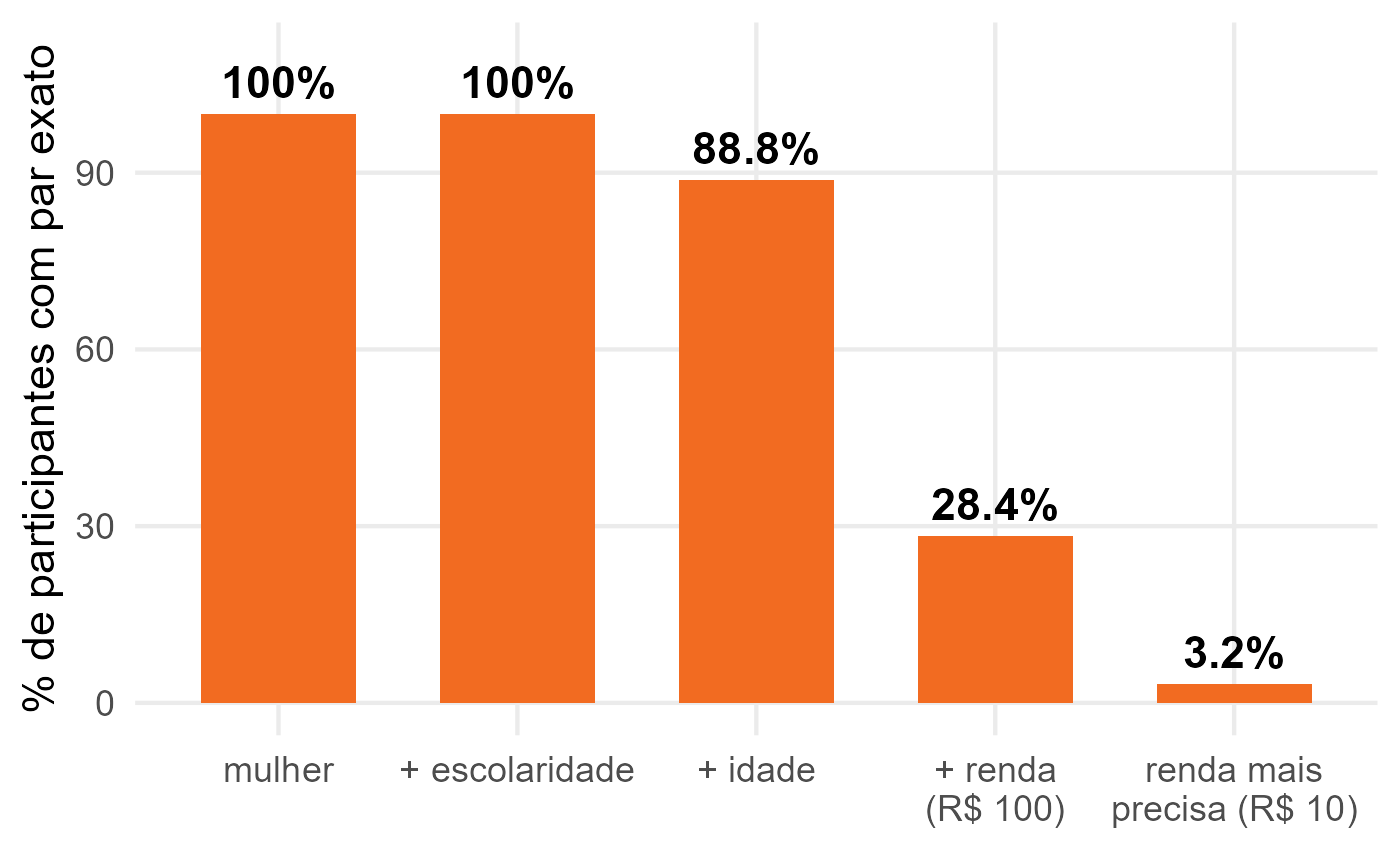
\includegraphics[height=3.9cm]{03_maldicao.png}\par
  \footnotesize Pareamento exato: cada nova variável derruba a chance de achar um ``gêmeo''. \textbf{Solução}: resumir tudo em um número, o \ind{propensity score} (probabilidade de participar), e parear por ele.
\end{frame}

\begin{frame}{Pareamento: características e exemplos}
  \carac{não participantes \textbf{parecidos} (mesmo escore de propensão)}
        {\textbf{sem confundidores não observados}; região comum (há semelhantes nos dois grupos)}
        {efeito sobre os tratados (ATT)}
        {muitas covariáveis \textbf{anteriores} ao programa (idealmente o resultado antes)}
        {política já implementada, sem sorteio, corte ou painel}
  \vspace{0.15cm}
  \textbf{\footnotesize\color{azul}Exemplos em políticas públicas}\par
    \scriptsize
    \begin{itemize}
      \item \textbf{Argentina:} programa de emprego Trabajar durante a crise de 1997 (Jalan e Ravallion, 2003).
      \item \textbf{Brasil:} Bolsa Família, efeitos sobre consumo, educação e saúde (MDS, 2007).
      \item \textbf{EUA:} programa de treinamento profissional reanalisado com PSM (LaLonde, 1986; Dehejia e Wahba, 1999).
      \item \textbf{Hipotético (nosso Qualifica):} programa já implementado, sem sorteio.
    \end{itemize}
  
\end{frame}

\begin{frame}{Passo a passo: pareamento (1 de 2)}
  \relax{\scriptsize\setlength{\tabcolsep}{2.5pt}\renewcommand{\arraystretch}{1.1}\begin{tabular}{@{}cP{2.55cm}P{2.75cm}P{3.6cm}@{}}
    \toprule
    \cabecalho{Como ler e decidir}
    \linha{1}{Compare os grupos \textbf{antes}: diferença simples e balanço (SMD)}{diferença = 587\newline SMD: escolaridade 0,50\newline renda antes 0,80\newline idade $-0{,}17$}{Grupos muito diferentes: a comparação simples \textbf{não vale}. É preciso ajustar.}
    \linha{2}{Estime o escore (logit) e olhe a \textbf{região comum}}{região comum:\newline 0,05 a 0,90}{Ampla sobreposição: há controles para quase todos. Se fosse estreita, o efeito valeria só para poucos.}
    \ultimalinha{3}{Pareie: vizinho mais próximo, \emph{caliper} de 0,2 dp}{1.630 de 1.631 tratados pareados}{Quase todos têm par. Muitos sem par $\Rightarrow$ o efeito vale só para os pareados.}
  \end{tabular}}
\end{frame}

\begin{frame}{Passo a passo: pareamento (2 de 2)}
  \relax{\scriptsize\setlength{\tabcolsep}{2.5pt}\renewcommand{\arraystretch}{1.1}\begin{tabular}{@{}cP{2.55cm}P{2.75cm}P{3.6cm}@{}}
    \toprule
    \cabecalho{Como ler e decidir}
    \linha{4}{\textbf{Balanço depois} do pareamento}{SMD: escolaridade $-0{,}03$\newline idade 0,01; renda antes 0,00\newline motivação 0,30}{Observáveis equilibradas ($<$ 0,10). A \textbf{motivação} (não observada) ainda difere.}
    \linha{5}{Estime o \textbf{ATT} e o intervalo (\emph{bootstrap})}{ATT = 297\newline EP = 8,8\newline IC 95\%: 280 a 315}{Participantes ganham ${\approx}$ R\$ 297 a mais por causa do programa (verdade: 300).}
    \ultimalinha{6}{\textbf{Robustez}: refaça sem a renda antes}{ATT = 476}{Muda muito: depende de uma covariável-chave. Relate e discuta o que pode estar omitido.}
  \end{tabular}}
  \caixaconclusao{o PSM só iguala o que está no modelo.}
\end{frame}

\begin{frame}{Região comum e resultado}
  \begin{columns}[T]
    \begin{column}{0.48\textwidth}
      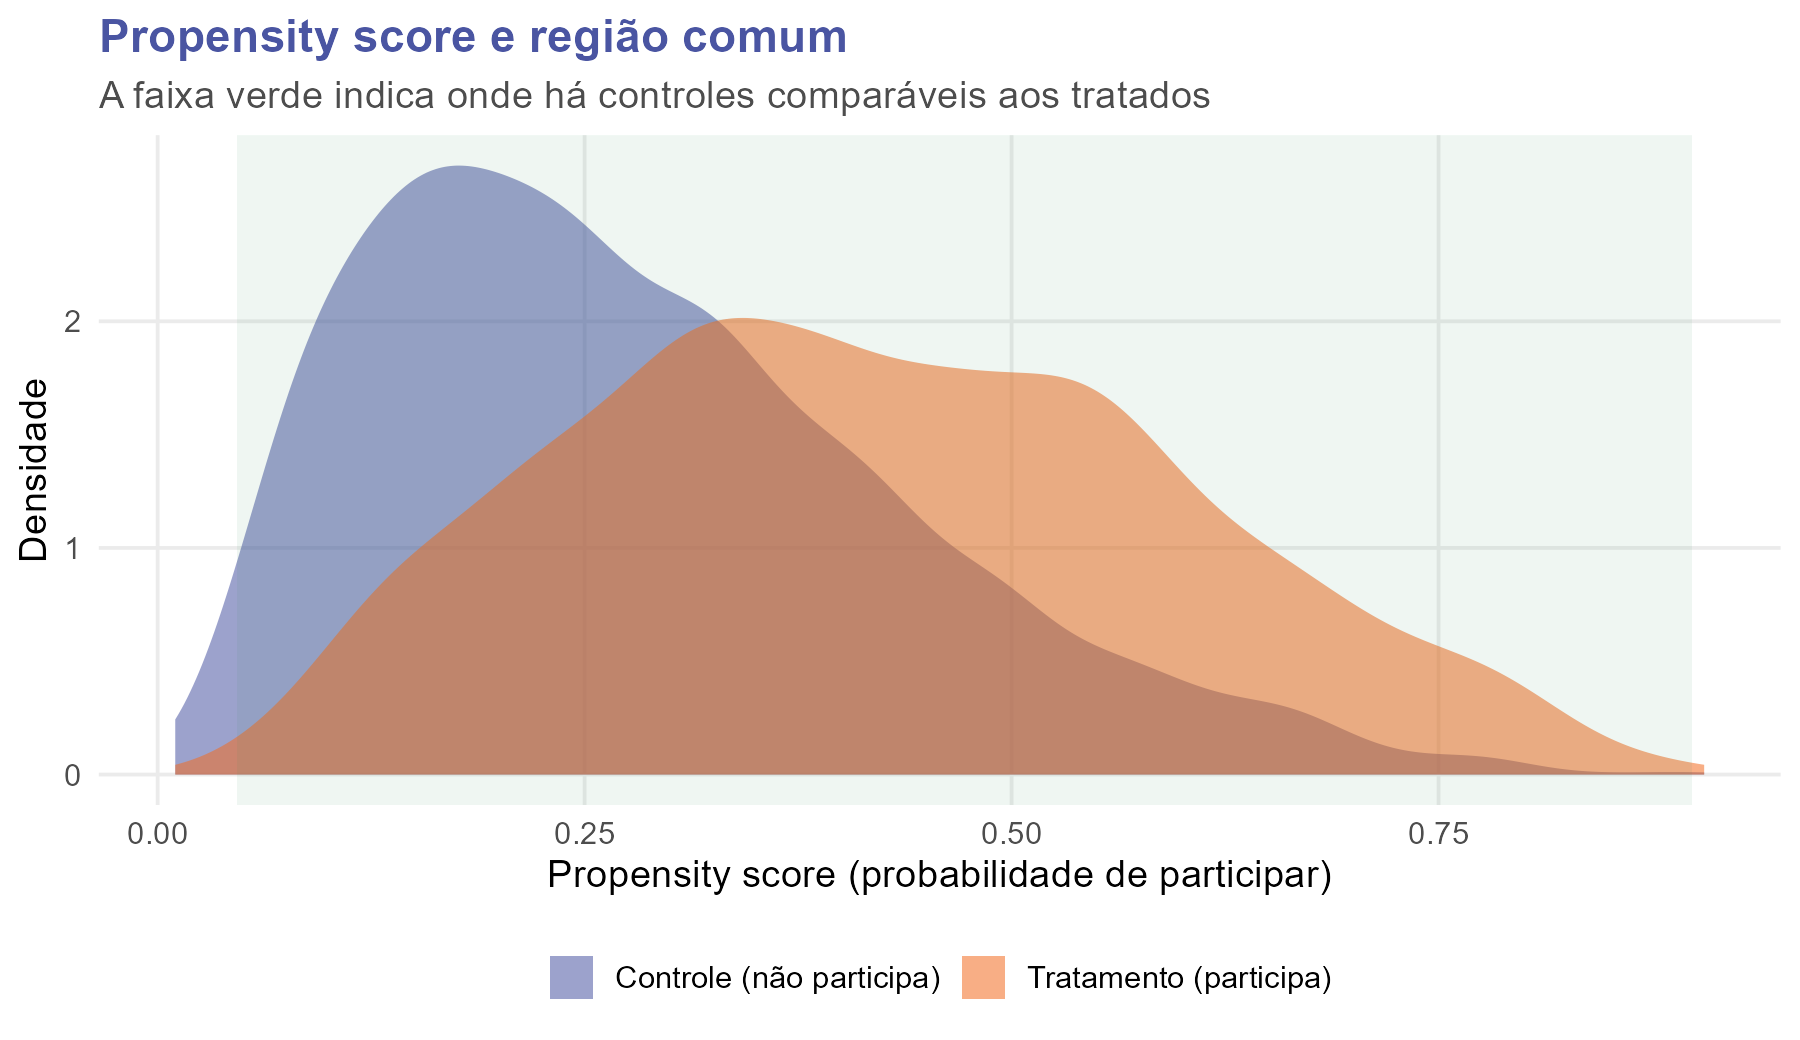
\includegraphics[height=3.2cm]{03_regiao_comum.png}\par
      {\tiny Faixa verde: onde há controles comparáveis.}
    \end{column}
    \begin{column}{0.52\textwidth}
      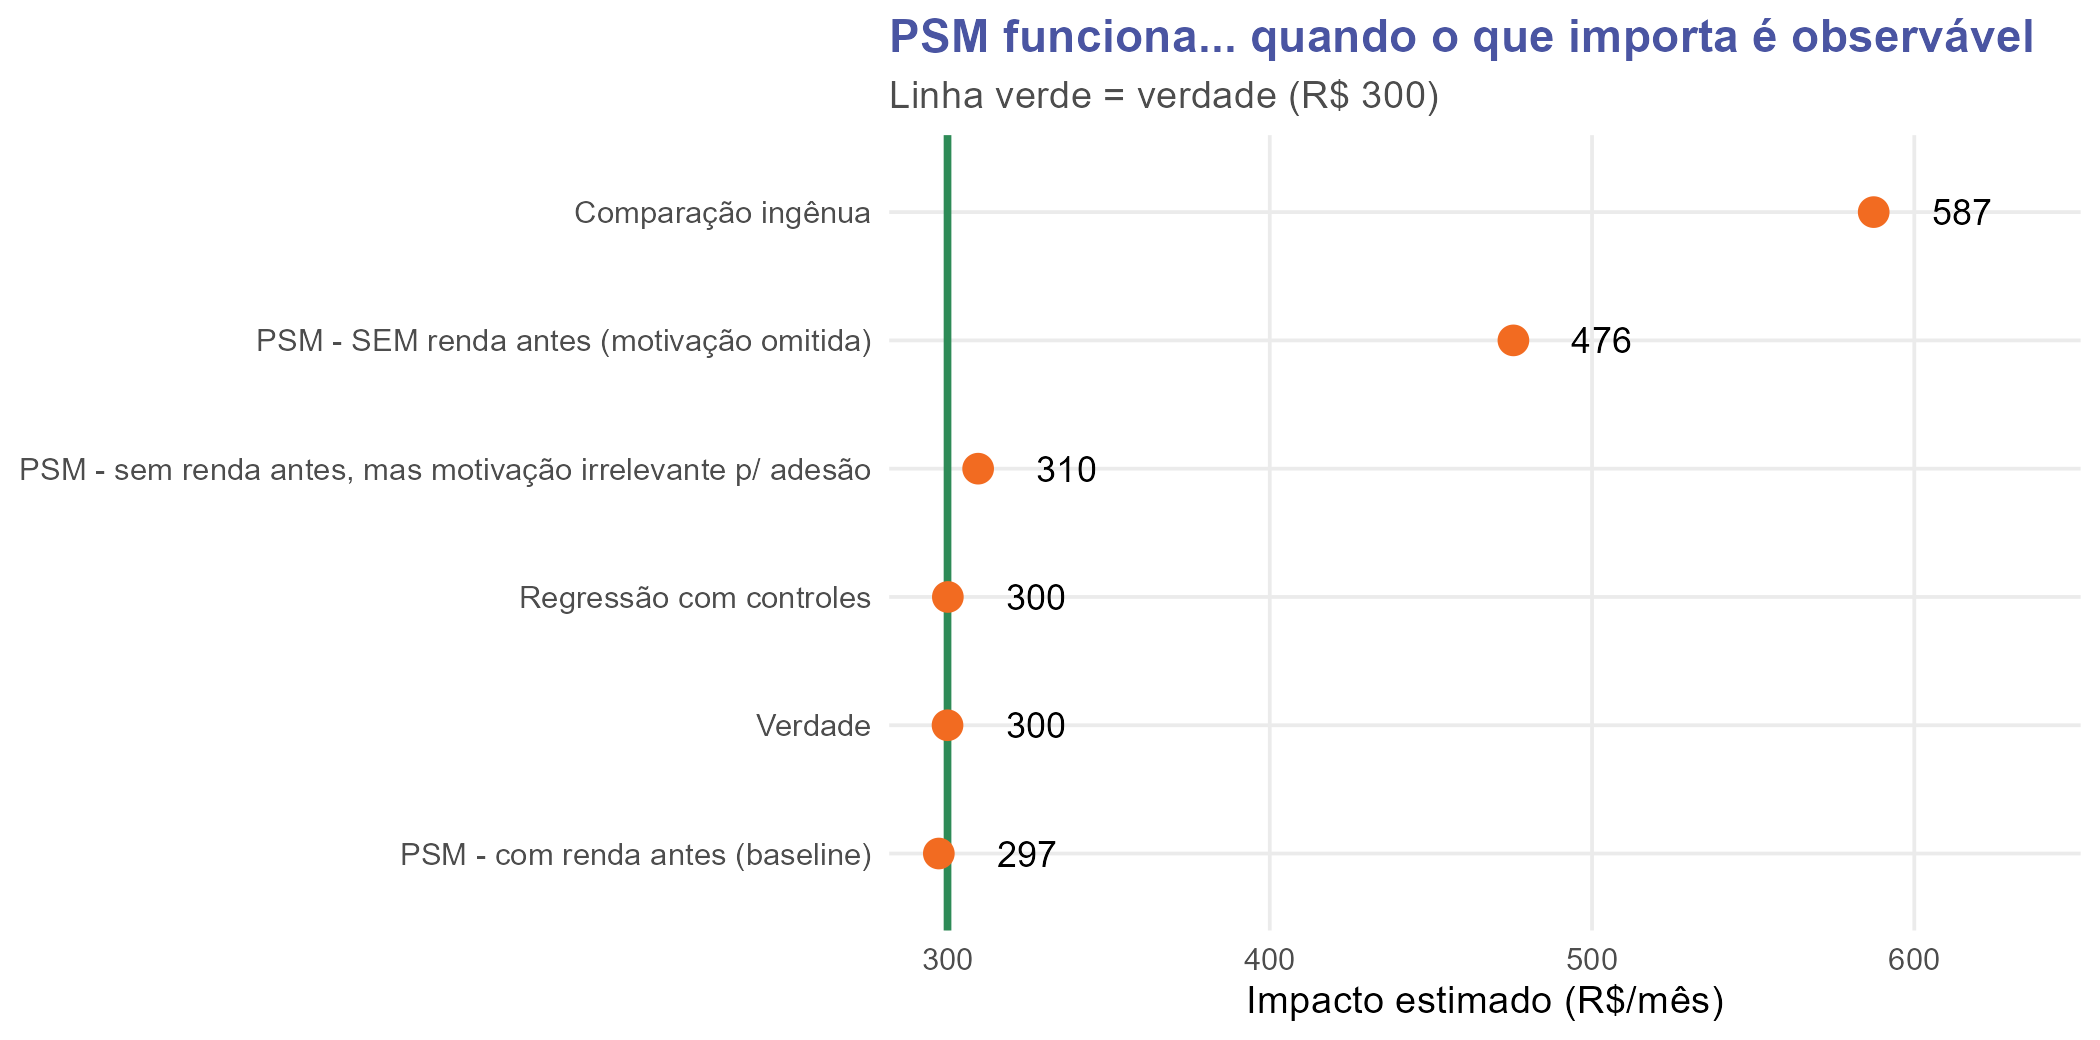
\includegraphics[height=3.2cm]{03_resumo.png}\par
      {\tiny Linha verde: verdade (R\$ 300).}
    \end{column}
  \end{columns}
\end{frame}
